% Provenance (never printed): see sources/outline_sources.md (Year 2: anatexis, migmatites,
% granite types and their sources). Wet granite solidus from Stern and Wyllie (1981) and
% Boettcher and Wyllie (1968); dehydration-melting brackets from Patino Douce and Harris
% (1998), Berger and Kalt (1999), Skjerlie and Johnston (1996); water solubility from Holtz
% et al. (1995); migmatite terms from the IUGS-SCMR proposal and BGS RR 99-02; aluminosity
% after Shand (as given by Moyen et al. 2017); figure data in figdata/bachelor-2/anatexis.py
% (paths from ptpaths.py); exercise and problem values in the Book 4 scratch calculator
% calc/ch12.py.
\chapter{انصهار القشرة: الميغماتيت والغرانيت}\label{ch:b2:crustal-melting}

الغرانيت هو ما يجعل القارات خفيفة، والوشاح لا يستطيع أن يصنعه مباشرة: فصهارات
\omterm{def:b2:mantle-melting:peridotites}{البيريدوتيت} بازلتية. ومعظم الغرانيت هو القشرة القارية تصهر نفسها.
فحين يسخن جذر جبلي مثخن، أو حين يتجمّع البازلت تحت القشرة، أو حين يصعد صخر
ساخن فينخفض ضغطه، تتخلّى الميكا والأمفيبولات في القشرة العميقة عن
مائها، وتظهر صهارة غرانيتية بين الحبيبات، ويصير الصخر
ميغماتيتًا، نصفه متحوّل ونصفه ناري. يتتبّع هذا الفصل تلك \omterm{def:b2:magma-emplacement:magma}{الصهارة} من أولى
أغشيتها حتى \omterm{def:b2:magma-emplacement:bodies}{البلوتون} الذي قد تبنيه، ويقرأ في كيمياء الغرانيت الصخر الذي جاء
منه.

\begin{recall}
\textbf{من مجلد المرحلة الثانوية}: الغرانيت والغرانيتويد والغرانوديوريت؛ والصخور الفلسية والمافية؛
وجذور الأحزمة الجبلية. \textbf{من مجلد السنة الأولى}: إنتاج الحرارة الإشعاعي
المنشأ في القشرة؛ وحلمأة السيليكات والمعادن الطينية. \textbf{من كتب الكيمياء}: خط الصلابة وخط السيولة
لنظام ثنائي، والكتلة المولية وكمية المادة. \textbf{من
\cref{ch:b2:magma-emplacement}}: القواطع والبلوتونات والقباب الصهارية. \textbf{من
\cref{ch:b2:mantle-melting}}: \omterm{def:b2:mantle-melting:melting}{الانصهار الجزئي}، \omterm{def:b2:mantle-melting:peritectic}{والانصهار غير المتطابق}، والانصهار
بانخفاض الضغط. \textbf{من \cref{ch:b2:metamorphic-facies}}: \omterm{def:b2:metamorphic-facies:protoliths}{الميتابيليت}، \omterm{def:b2:metamorphic-facies:clapeyron}{وميل كلابيرون}
لتفاعل، والسحنات. \textbf{من \cref{ch:b2:pt-paths}}: \omterm{def:b2:pt-paths:ptt}{مسارات الضغط--الحرارة--الزمن}
ونموذج إثخان القشرة.
\end{recall}

\section{لماذا تنصهر القشرة}\label{sec:b2:crustal-melting:why}

للظاهرة اسم قديم وبسيط.

\begin{definition}[الأناتكسيس]\label{def:b2:crustal-melting:anatexis}
\emph{الأناتكسيس}\index{الأناتكسيس} هو انصهار صخر، أيًّا كانت درجة الانصهار؛
وفي الممارسة تُستعمل الكلمة للانصهار الجزئي للقشرة القارية.
\end{definition}
% ledger: scmr:migmatite

\subsection*{خط الصلابة الرطب}

لا ينصهر الغرانيت عند درجة حرارة منخفضة إلا إذا كان رطبًا. فقد صهر ستيرن وويلي غرانيتًا
بيوتيتيًا من باثوليث سييرا نيفادا مع فائض من الماء: فظهر أول سائل عند
\qty{680}{\celsius} تحت \qty{2}{kbar} وعند \qty{620}{\celsius} تحت \qty{10}{kbar}،
وانصهر الصخر كله على ارتفاع \qty{35}{\celsius} فقط فوق خط الصلابة تحت \qty{2}{kbar}، لكن على ارتفاع
\qty{105}{\celsius} فوقه تحت \qty{10}{kbar}. والغرانيت نفسه الذي درسه قبل ذلك
بوتشر وويلي بدأ ينصهر عند \qty{605}{\celsius} تحت \qty{15.3}{kbar}؛ وقرب
\qty{17}{kbar} تفكّك بلاجيوكليزه إلى جاديت وكوارتز، ومن هناك
انعطف خط الصلابة صاعدًا من جديد، فبلغ \qty{670}{\celsius} تحت \qty{27}{kbar}.
% ledger: sw81:wet-solidus, bw68:wet-solidus

ينخفض خط الصلابة الرطب كلما ارتفع الضغط، على عكس خط الصلابة الجاف. والسبب هو أين
يذهب الماء. فالماء الحرّ مائع منخفض الكثافة؛ أمّا إذا ذاب في \omterm{def:b2:magma-emplacement:magma}{الصهارة} فلا يشغل إلا
حيّزًا ضئيلًا: فقد وجد هولتس ومعاونوه حجمه المولي الجزئي في صهارة غرانيتية قريبًا
من \qtyrange{10}{12}{\cubic\centi\metre\per\mole}، مقابل \qty{18}{\cubic\centi\metre\per\mole}
للماء السائل في ظروف الغرفة وأكثر لمائع ساخن. فتفاعل الانصهار
\[\text{كوارتز} + \text{فلسبارات} + \ce{H2O}\ (\text{مائع}) \longrightarrow
\text{صهارة مائية}\]
له إذن تغيّر حجم سالب، بينما تغيّر إنتروبياه، كما في كل انصهار،
موجب: فبعلاقة كلابيرون في \cref{ch:b2:metamorphic-facies}، يكون ميله
$\mathrm{d}P/\mathrm{d}T = \Delta S/\Delta V$ سالبًا. ويُدخل الضغط أيضًا مزيدًا من الماء
في \omterm{def:b2:magma-emplacement:magma}{الصهارة}: ففي صهارة هابلوغرانيتية عند \qty{800}{\celsius} يرتفع محتوى التشبّع
من \qty{2.80}{\percent} كتليًا تحت \qty{0.5}{kbar} إلى \qty{9.97}{\percent} تحت
\qty{5}{kbar} و\qty{13.82}{\percent} تحت \qty{8}{kbar}، أي بزيادة نحو \qty{1.27}{\percent}
لكل كيلوبار بين 3 و\qty{8}{kbar}.
% ledger: holtz95:solubility

\begin{omfigure}
\centering
\begin{tikzpicture}
\begin{axis}[omrecord, width=0.5\linewidth, height=4.8cm,
  xmin=0, xmax=9, ymin=0, ymax=15, xlabel={\mbox{\textdir TLT $P$ (\unit{kbar})}},
  ylabel={نسبة \ce{H2O} في الصهارة \babelsublr{(\unit{\percent})}},
  tick label style={font=\scriptsize}, label style={font=\small}]
\addplot[only marks, mark=*, mark size=1.6pt, blue!70!black]
  table[x=P_kbar, y=H2O_wt] {figdata/out/bachelor-2-anatexis-water.dat};
\addplot[thick, red!75!black] table[x=P_kbar, y=H2O_wt] {figdata/out/bachelor-2-anatexis-waterfit.dat};
\end{axis}
\end{tikzpicture}
\par\smallskip{\small الماء الذي تستطيع صهارة هابلوغرانيتية إذابته عند \qty{800}{\celsius}
(نقاط مقيسة)؛ وبالأحمر: خط المربعات الصغرى عبر النقاط من 3 إلى
\qty{8}{kbar}، وميله \qty{1.26}{\percent} لكل كيلوبار.}
\end{omfigure}
% ledger: holtz95:solubility

لكن القشرة العميقة لا تحوي إلا قليلًا من الماء الحرّ: فالصخر المتحوّل الذي سُخّن قد
طرد معظم ماء مسامّه، عبر تفاعلات نزع الماء في
\cref{ch:b2:metamorphic-facies}. وماؤه الآن محبوس في الميكا والأمفيبولات. فعلى الانصهار
إذن أن ينتظر تفكّك هذه المعادن نفسها.

\begin{definition}[الانصهار بحضور مائع وانصهار نزع الماء]\label{def:b2:crustal-melting:reactions}
\emph{الانصهار بحضور مائع}\index{الانصهار بحضور مائع} (أو الانصهار بتدفّق الماء) هو
الانصهار في وجود مائع مائي حرّ، عند خط الصلابة الرطب أو قربه؛ وكمية \omterm{def:b2:magma-emplacement:magma}{الصهارة}
الناتجة محدودة بما يتوفّر من المائع. و\emph{انصهار نزع الماء}\index{انصهار نزع الماء}
(الانصهار في غياب المائع) هو \omterm{def:b2:mantle-melting:peritectic}{الانصهار غير المتطابق} لمعدن مائي، ميكا أو
أمفيبول، مع الكوارتز والفلسبار، دون أيّ مائع حرّ: فيدخل ماء المعدن
\omterm{def:b2:magma-emplacement:magma}{الصهارة}، وتنمو بجانبها معادن لامائية جديدة (فلسبار بوتاسي بيريتكتي، وسيليكات ألومنيوم،
وغارنت، وكورديريت، وأورثوبيروكسين).
\end{definition}
% ledger: pj98:productivity, koester02:melting, pdh98:himalaya

تثبّت التجارب أين يستسلم كل معدن مائي. ففي شيستات المسكوفيت من
الهيمالايا، وجد باتينيو دوس وهاريس أن \omterm{def:b2:crustal-melting:reactions}{انصهار نزع الماء} يبدأ عند 750 إلى
\qty{800}{\celsius} بين 6 و\qty{10}{kbar}؛ وإضافة الماء إلى الصخور نفسها خفضت
خط الصلابة لكنها أعطت صهارات ترونجيمية لا تشبه \omterm{def:b2:crustal-melting:leucogranite}{الليوكوغرانيت}. وبدأ نيس شبه طيني
ينصهر قرب \qty{700}{\celsius} عبر مسكوفيته الفينغيتي، لكنه أنتج أقل
من \qty{9}{\percent} من \omterm{def:b2:magma-emplacement:magma}{الصهارة}؛ وفوق \qty{800}{\celsius}، أعطى تفكّك البيوتيت
والكورديريت من 10 إلى \qty{63}{\percent} حجميًا. وجرى \omterm{def:b2:crustal-melting:reactions}{انصهار نزع الماء} من البيوتيت
عند 800 إلى \qty{850}{\celsius} و0.5 إلى \qty{0.7}{GPa} في ميغماتيتات
الغابة البافارية، ويضيف الأمفيبول نحو \qty{25}{\percent} من \omterm{def:b2:magma-emplacement:magma}{الصهارة} حجميًا بين 875
و\qty{925}{\celsius} تحت 10 إلى \qty{12.5}{kbar}. والترتيب هو ترتيب تمسّك المعادن بالماء:
المسكوفيت أولًا، ثم البيوتيت، والأمفيبول أخيرًا.
% ledger: pdh98:himalaya, koester02:melting, bk99:migmatites, sj96:amphibole, moyen17:aluminosity

\begin{proposition}[نسبة صهارة يحدّها الماء]\label{prop:b2:crustal-melting:water}
في \omterm{def:b2:crustal-melting:reactions}{انصهار نزع الماء} دون أيّ مائع حرّ، إذا حوى صخر نسبة كتلية $X$ من
معدن مائي يحتوي نسبة كتلية $w$ من الماء، ودخل كل هذا الماء
صهارة تحوي نسبة كتلية $c$ من الماء، فإن النسبة الكتلية للصهارة هي
\[F = \frac{X\,w}{c}.\]
ولأن $c$ لا يمكن أن تتجاوز محتوى التشبّع $c_{\mathrm{sat}}$ عند ضغط الانصهار
ودرجة حرارته، فإن $F \ge X\,w/c_{\mathrm{sat}}$: فكلما قلّ الماء الذي تحويه \omterm{def:b2:magma-emplacement:magma}{الصهارة}، زادت
\omterm{def:b2:magma-emplacement:magma}{الصهارة} التي تصنعها الميكا نفسها.
\end{proposition}

\begin{proof}
لكل كيلوغرام من الصخر يحرّر المعدن $X\,w$ كيلوغرامًا من الماء. ومع انعدام الطور المائع
وعدم بقاء ماء في المواد الصلبة، يكون كله في \omterm{def:b2:magma-emplacement:magma}{الصهارة}، التي تحوي كتلتها $F$ مقدار $c\,F$
كيلوغرامًا من الماء: $c\,F = X\,w$. وبما أن $c \le c_{\mathrm{sat}}$، فإن $F = Xw/c \ge
Xw/c_{\mathrm{sat}}$.
\end{proof}

المسكوفيت، \ce{KAl3Si3O10(OH)2} ذو الكتلة المولية \qty{398.3}{\gram\per\mole}، يحوي مجموعتي
هيدروكسيل، أي ما يعادل جزيء ماء واحدًا، أو \qty{4.52}{\percent} من
كتلته. فالشيست الذي فيه \qty{20}{\percent} مسكوفيت لديه إذن \qty{9.0}{\gram} من الماء
لكل كيلوغرام يتخلّى عنها؛ فإذا ذابت بنسبة \qty{6}{\percent}، صنعت \qty{150}{\gram} من
\omterm{def:b2:magma-emplacement:magma}{الصهارة}. فالميكا تحدّد الميزانية، ولهذا تكون القشرة الخصبة، أي القشرة التي تنصهر بسهولة،
غنية بالميكا: \omterm{def:b2:metamorphic-facies:protoliths}{والميتابيليت} في مقدّمتها.

\begin{omfigure}
\centering
\begin{tikzpicture}
\begin{axis}[omrecord, width=0.8\linewidth, height=7cm,
  xmin=500, xmax=1000, ymin=0, ymax=20, xlabel={\mbox{\textdir TLT $T$ (\unit{\celsius})}}, ylabel={\mbox{\textdir TLT $P$ (\unit{kbar})}},
  tick label style={font=\scriptsize}, label style={font=\small}, clip=false]
\addplot[fill=orange!35, draw=orange!70!black] coordinates {(750,6) (800,6) (800,10) (750,10) (750,6)};
\addplot[fill=red!25, draw=red!70!black] coordinates {(800,5) (850,5) (850,7) (800,7) (800,5)};
\addplot[fill=green!25, draw=green!50!black] coordinates {(875,10) (925,10) (925,12.5) (875,12.5) (875,10)};
\node[font=\scriptsize, orange!50!black, align=center] at (axis cs:775,8) {مسكوفيت};
\node[font=\scriptsize, red!60!black] at (axis cs:825,4.4) {بيوتيت};
\node[font=\scriptsize, green!35!black, anchor=west] at (axis cs:927,11.25) {أمفيبول};
\addplot[very thick, blue!70!black, mark=*, mark size=1.5pt]
  table[x=T_C, y=P_kbar] {figdata/out/bachelor-2-anatexis-solidi.dat};
\node[font=\scriptsize, blue!70!black, anchor=west] at (axis cs:612,15.6) {خط صلابة الغرانيت الرطب};
\addplot[thick, black, postaction={decorate}, decoration={markings,
  mark=at position 0.3 with {\arrow{>}}, mark=at position 0.75 with {\arrow{>}}}]
  table[x=T_C, y=P_kbar, restrict x to domain=500:1000,
  restrict expr to domain={\thisrow{t_Myr}}{0:100}] {figdata/out/bachelor-2-anatexis-path35.dat};
\node[font=\scriptsize, anchor=north] at (axis cs:560,4.2) {\foreignlanguage{arabic}{صخر من عمق \qty{35}{km}}};
\addplot[thick, dashed, black, postaction={decorate}, decoration={markings,
  mark=at position 0.3 with {\arrow{>}}, mark=at position 0.7 with {\arrow{>}}}]
  table[x=T_C, y=P_kbar, restrict x to domain=500:1000,
  restrict expr to domain={\thisrow{t_Myr}}{0:100}] {figdata/out/bachelor-2-anatexis-path70.dat};
\node[font=\scriptsize, anchor=south] at (axis cs:760,19.4) {قاعدة القشرة المثخنة};
\end{axis}
\end{tikzpicture}
\par\smallskip{\small أين تنصهر القشرة. بالأزرق: خط صلابة غرانيت بيوتيتي مع
فائض من الماء (نقاط مقيسة، موصولة بقطع مستقيمة). والمستطيلات: الظروف التي
رُصد عندها \omterm{def:b2:crustal-melting:reactions}{انصهار نزع الماء} من المسكوفيت والبيوتيت والأمفيبول في التجارب وفي
\omterm{def:b2:crustal-melting:migmatite}{الميغماتيت}. وبالأسود: مسارات محسوبة بنموذج الإثخان في
\cref{ch:b2:pt-paths}؛ فالصخر الذي ينتهي على عمق \qty{35}{km} بعد التكديس (المتّصل) لا
يبلغ أبدًا خط الصلابة الرطب، بينما تتجاوز قاعدة القشرة المثخنة (المتقطّع)
\qty{900}{\celsius}. والمساران مرسومان لأول 100 مليون سنة، حتى
يتوقّف الحتّ.}
\end{omfigure}
% ledger: sw81:wet-solidus, bw68:wet-solidus, pdh98:himalaya, bk99:migmatites, sj96:amphibole, et84:ptt

\subsection*{من أين تأتي الحرارة}

يطرح الشكل أعلاه المسألة: فالقشرة لا تنصهر إلا حيث تكون أسخن من نحو
\qty{700}{\celsius}، بينما لا يبلغ التدرّج الحراري الأرضي المستقر للنموذج في \cref{ch:b2:pt-paths}
إلا \qty{595}{\celsius} عند قاعدة قشرة سمكها \qty{35}{km}. وثلاث طرق تقود
إلى ما بعد تفاعلات \omterm{def:b2:crustal-melting:reactions}{انصهار نزع الماء}.

\emph{الإثخان والحرارة الإشعاعية المنشأ.} في نموذج \cref{ch:b2:pt-paths}، تسخن قشرة
مضاعفة بالتكديس من داخلها؛ فالصخر الذي ينتهي على عمق منتصف القشرة يبلغ ذروته عند
\qty{593}{\celsius} ولا ينصهر أبدًا، لكن قاعدة القشرة المثخنة تتجاوز
\qty{800}{\celsius} بعد نحو 31 مليون سنة و\qty{900}{\celsius} بعد نحو 56، أي بعد
تفاعل البيوتيت. فانصهار القشرة السفلى نتيجة بطيئة للإثخان.
% ledger: et84:ptt

\emph{انخفاض الضغط.} الصخر الساخن الذي يُرفع أسرع مما يبرد يعبر
منحنيات \omterm{def:b2:crustal-melting:reactions}{انصهار نزع الماء} من جهة الضغط المرتفع. وقد وجد باتينيو دوس وهاريس أن
لخط صلابة شيست المسكوفيت قيمة $\mathrm{d}P/\mathrm{d}T$ أصغر من قيمة
شيست البيوتيت، فينصهر شيست المسكوفيت بسهولة أكبر عند انخفاض الضغط،
واستنتجا أن \omterm{def:b2:crustal-melting:leucogranite}{الليوكوغرانيت} الهيمالايي تكوّن \omterm{def:b2:crustal-melting:reactions}{بانصهار نزع الماء} من \omterm{def:b2:metamorphic-facies:protoliths}{الميتابيليت}
أثناء انخفاض كظوم للضغط عند 6 إلى \qty{8}{kbar} و750 إلى \qty{770}{\celsius}.
% ledger: pdh98:himalaya

\emph{الحرارة من الأسفل.} البازلت الآتي من الوشاح الذي يتوقّف عند قاعدة القشرة يجلب
معه حرارته وحرارته الكامنة للتبلور.

\begin{definition}[التبطين المافي]\label{def:b2:crustal-melting:underplating}
\emph{التبطين المافي}\index{التبطين المافي} هو تجمّع صهارة بازلتية
آتية من الوشاح عند قاعدة القشرة القارية أو قربها، حيث تتبلور
وتحرّر حرارتها في القشرة التي فوقها.
\end{definition}

استُند إلى التبطين، مثلًا، لتفسير الريوليت في شبه جزيرة القارة القطبية الجنوبية،
حيث جاءت صهارة أنديزيتية إلى داسيتية من انصهار قشرة سفلى مافية مائية
استجابةً للتبطين؛ ويمكن لصهارات الوشاح أيضًا أن تصنع الغرانيتويدات نفسها، بالتبلور
أو بإعادة صهر أجسام مبطَّنة حديثًا.
% ledger: riley01:underplating, moyen17:settings, johansson23:a-type

\begin{proposition}[الميزانية الحرارية للتبطين]\label{prop:b2:crustal-melting:heat}
حجم $V_b$ من البازلت متداخل عند $T_b$ يتبلور كليًا، فيحرّر
حرارة كامنة $L_b$ لكل وحدة حجم، ويبرد إلى $T_f$، يستطيع أن يرفع حجمًا $V_c$ من القشرة
من $T_c$ إلى $T_f$ وأن يصهر نسبة $F$ منه، حيث
\[\frac{V_c}{V_b} = \frac{L_b + C\,(T_b - T_f)}{C\,(T_f - T_c) + F\,L_c},\]
حيث $C$ السعة الحرارية لكل وحدة حجم (مأخوذة متساوية للصخرين) و$L_c$
الحرارة الكامنة لصهارة القشرة لكل وحدة حجم، إذا لم تُفقد أيّ حرارة.
\end{proposition}

\begin{proof}
الحرارة التي يحرّرها البازلت، $V_b[L_b + C(T_b - T_f)]$، تساوي الحرارة التي تمتصّها
القشرة، $V_c[C(T_f - T_c) + F L_c]$؛ اقسم على $V_b$ وعلى قوس القشرة.
\end{proof}

مع $C = \qty{2.5}{\mega\joule\per\cubic\metre\per\kelvin}$ وحرارات كامنة قدرها
\qty{900}{\mega\joule\per\cubic\metre}، وهي قيم نموذجية للصهارات، يستطيع بازلت يبرد من
\qty{1200}{\celsius} إلى \qty{850}{\celsius} أن يسخّن نحو مرتين ونصف حجمه
من القشرة انطلاقًا من \qty{650}{\celsius} وأن يصهر خُمسها (\cref{exo:b2:crustal-melting:7}).
فالتبطين فعّال، لكنه محلّي: فالحرارة تذهب حيث يكون البازلت.
% ledger: delaney86b4:properties

\section{الأناتكسيس والميغماتيت}\label{sec:b2:crustal-melting:migmatites}

الصخر المنصهر جزئيًا الذي يتجمّد قبل أن تغادره صهارته يحتفظ بالجزأين جنبًا إلى جنب.

\begin{definition}[الميغماتيت وأجزاؤه]\label{def:b2:crustal-melting:migmatite}
\emph{الميغماتيت}\index{الميغماتيت} صخر سيليكاتي مركّب، غير متجانس على
مقياس المكشف، مكوّن من أجزاء أدكن لها مظهر صخر متحوّل وأجزاء أفتح
ذات مظهر بلوتوني. و\emph{الليوكوسوم}\index{الليوكوسوم} هو جزؤه الفاتح الغني بالكوارتز
والفلسبار؛ و\emph{الميلانوسوم}\index{الميلانوسوم} جزؤه الداكن، الغني بالمعادن
الداكنة، والمكمّل لليوكوسوم؛ و\emph{الميزوسوم} الجزء ذو اللون
المتوسط، وهو بقية معدّلة قليلًا أو كثيرًا من الصخر الأم (\emph{الباليوسوم}).
ويشكّل الليوكوسوم والميلانوسوم معًا \emph{النيوسوم}، أي الجزء المتكوّن حديثًا.
و\emph{الميتاتكسيت}\index{الميتاتكسيت} ميغماتيت ذو ليوكوسومات وميزوسومات وميلانوسومات منفصلة
ومحدّدة جيدًا؛ و\emph{الدياتكسيت}\index{الدياتكسيت} ميغماتيت تندمج فيه الأجزاء الفاتحة
والداكنة في خطوط (شليرن) وبنى شبحية (سديمية).
\end{definition}
% ledger: scmr:migmatite, bgs99:migmatite

التعريف وصفيّ عن قصد: فكون \omterm{def:b2:crustal-melting:migmatite}{الليوكوسوم} صهارة متجمّدة، أو صهارة
جاءت من مكان آخر، أو انفصالًا تحوّليًا، هو تفسير. فحين يكون
صهارة، يكون \omterm{def:b2:crustal-melting:migmatite}{الليوكوسوم} هو السائل \omterm{def:b2:crustal-melting:migmatite}{والميلانوسوم} البقية الصلبة التي تركها، المغتنية
بالبيوتيت أو الغارنت أو الكورديريت: \omterm{def:b2:crustal-melting:migmatite}{فالميتاتكسيت} يسجّل المرحلة الأولى من \omterm{def:b2:crustal-melting:anatexis}{الأناتكسيس}، حيث
لم ينصهر إلا جزء من الصخر، \omterm{def:b2:crustal-melting:migmatite}{والدياتكسيت} مرحلة متقدّمة، حيث انصهرت المعادن الداكنة
أيضًا وبقيت \omterm{def:b2:magma-emplacement:magma}{الصهارة} في مكانها.
% ledger: scmr:migmatite

كم من \omterm{def:b2:magma-emplacement:magma}{الصهارة} في \omterm{def:b2:crustal-melting:migmatite}{الميغماتيت}؟ في ميغماتيتات الكورديريت في الغابة البافارية،
المتكوّنة \omterm{def:b2:crustal-melting:reactions}{بانصهار نزع الماء} من البيوتيت، تشكّل الليوكوسومات التي هي صهارة سابقة خالصة من 20 إلى
\qty{40}{\percent} من الصخر حجميًا، قريبًا من 20 إلى \qty{30}{\percent} الناتجة في
تجارب \omterm{def:b2:crustal-melting:reactions}{انصهار نزع الماء} على صخور مماثلة في الظروف نفسها؛ وحيث
أُزيلت \omterm{def:b2:magma-emplacement:magma}{الصهارة}، كما في الأنواع الأشدّ تشوّهًا، تبقى البقية خلفها.
% ledger: bk99:migmatites

\begin{inthefield}[قراءة مكشف ميغماتيتي]
على مكشف ميغماتيتي يرسم الجيولوجي أولًا خريطة الأجزاء وهندستها: هل تقع
الليوكوسومات في التورّق أم تقطعه، وهل تحمل حافة داكنة ميلانوقراطية،
وكم من \omterm{def:b2:crustal-melting:migmatite}{الميلانوسوم} يقابل كل ليوكوسوم. ولكل سمة معنى. فالصخر المتبقّي
الميلانوقراطي يدلّ على المكان الذي جاءت منه \omterm{def:b2:magma-emplacement:magma}{الصهارة}؛ والليوكوسومات الرقيقة القصيرة المتفرّعة ذات
\omterm{def:b2:crustal-melting:migmatite}{الميلانوسوم} القليل تدلّ على انصهار بدأ للتوّ؛ والليوكوسومات الموازية للتورّق
تدلّ على المكان الذي صُرّفت فيه \omterm{def:b2:magma-emplacement:magma}{الصهارة} من الأرضية وتجمّعت؛ والليوكوسومات التي تصنع زاوية كبيرة مع
التطبّق، وعادةً بلا حواف داكنة، تكوّنت أخيرًا وتدلّ على القنوات التي
غادرت عبرها \omterm{def:b2:magma-emplacement:magma}{الصهارة}. والنسبة المرتفعة للميلانوسوم إلى \omterm{def:b2:crustal-melting:migmatite}{الليوكوسوم} تعني أن معظم \omterm{def:b2:magma-emplacement:magma}{الصهارة} قد ذهب.
ثم تؤخذ عيّنات من \omterm{def:b2:crustal-melting:migmatite}{الليوكوسوم} \omterm{def:b2:crustal-melting:migmatite}{والميلانوسوم} والميزوسوم للتحليل، لاختبار ما إذا كان المكشف
قد فقد صهارة، بموازنة الكتلة (\cref{exo:b2:crustal-melting:12}).
\end{inthefield}
% ledger: sawyer01:segregation, bgs99:migmatite, scmr:migmatite

\begin{omfigure}
\centering
\begin{tikzpicture}[x=1cm, y=1cm]
% (a) stromatic
\begin{scope}
\fill[gray!45] (0,0) rectangle (3,3);
\foreach \y in {0.45, 1.25, 2.05, 2.7} {
  \fill[black!70] (0,\y-0.2) .. controls (1,\y-0.15) and (2,\y-0.25) .. (3,\y-0.2)
    -- (3,\y+0.2) .. controls (2,\y+0.15) and (1,\y+0.25) .. (0,\y+0.2) -- cycle;
  \fill[white] (0,\y-0.14) .. controls (1,\y-0.09) and (2,\y-0.19) .. (3,\y-0.14)
    -- (3,\y+0.14) .. controls (2,\y+0.09) and (1,\y+0.19) .. (0,\y+0.14) -- cycle;
}
\draw[thick] (0,0) rectangle (3,3);
\node[font=\small, anchor=north] at (1.5,-0.1) {\foreignlanguage{arabic}{(أ) ستروماتي}};
\end{scope}
% (b) agmatitic
\begin{scope}[xshift=3.4cm]
\fill[white] (0,0) rectangle (3,3);
\fill[gray!45, draw=black!70, thick] (0.15,0.15) -- (1.3,0.25) -- (1.2,1.25) -- (0.2,1.1) -- cycle;
\fill[gray!45, draw=black!70, thick] (1.5,0.2) -- (2.85,0.15) -- (2.8,1.0) -- (1.6,1.35) -- cycle;
\fill[gray!45, draw=black!70, thick] (0.2,1.35) -- (1.25,1.5) -- (1.4,2.8) -- (0.15,2.85) -- cycle;
\fill[gray!45, draw=black!70, thick] (1.65,1.6) -- (2.85,1.25) -- (2.85,2.85) -- (1.6,2.8) -- cycle;
\draw[thick] (0,0) rectangle (3,3);
\node[font=\small, anchor=north] at (1.5,-0.1) {\foreignlanguage{arabic}{(ب) أغماتيتي}};
\end{scope}
% (c) schlieric
\begin{scope}[xshift=6.8cm]
\fill[white] (0,0) rectangle (3,3);
\foreach \y/\a in {0.5/0.3, 1.1/-0.25, 1.7/0.2, 2.3/-0.3} {
  \draw[black!75, line width=1.4pt] (0.2,\y) .. controls (1,\y+\a) and (1.8,\y-\a) .. (2.8,\y+0.1);
}
\draw[black!60, line width=0.8pt] (0.6,2.75) .. controls (1.4,2.55) .. (2.4,2.8);
\draw[thick] (0,0) rectangle (3,3);
\node[font=\small, anchor=north] at (1.5,-0.1) {\foreignlanguage{arabic}{(ج) شليري}};
\end{scope}
% (d) nebulitic
\begin{scope}[xshift=10.2cm]
\fill[white] (0,0) rectangle (3,3);
\shade[inner color=gray!50, outer color=white] (0.9,1.0) ellipse (0.75 and 0.45);
\shade[inner color=gray!45, outer color=white] (2.1,2.1) ellipse (0.7 and 0.4);
\shade[inner color=gray!35, outer color=white] (2.2,0.7) ellipse (0.5 and 0.3);
\draw[thick] (0,0) rectangle (3,3);
\node[font=\small, anchor=north] at (1.5,-0.1) {\foreignlanguage{arabic}{(د) سديمي}};
\end{scope}
\end{tikzpicture}
\par\smallskip{\small أربع بنى للميغماتيت، تخطيطيًا (أوجه مكاشف عرضها نحو متر
واحد). الأبيض: \omterm{def:b2:crustal-melting:migmatite}{الليوكوسوم}؛ والأسود: \omterm{def:b2:crustal-melting:migmatite}{الميلانوسوم}؛ والرمادي: الميزوسوم. (أ) ستروماتي: طبقات من
\omterm{def:b2:crustal-melting:migmatite}{الليوكوسوم}، لكلٍّ منها حافة داكنة، موازية للتورّق، نموذجية للميتاتكسيت.
(ب) أغماتيتي: شبكة من عروق \omterm{def:b2:crustal-melting:migmatite}{الليوكوسوم} حول كتل زاويّة، تعطي مظهرًا
بريشيًا. (ج) شليري: خطوط من المعادن الداكنة داخل \omterm{def:b2:crustal-melting:migmatite}{الليوكوسوم}. (د) سديمي: أشباح
منتشرة من الصخر الأقدم في مضيف ذي مظهر ناري؛ و(ج) و(د) نموذجيتان
للدياتكسيت.}
\end{omfigure}
% ledger: bgs99:migmatite, scmr:migmatite

\begin{omfigure}
\centering
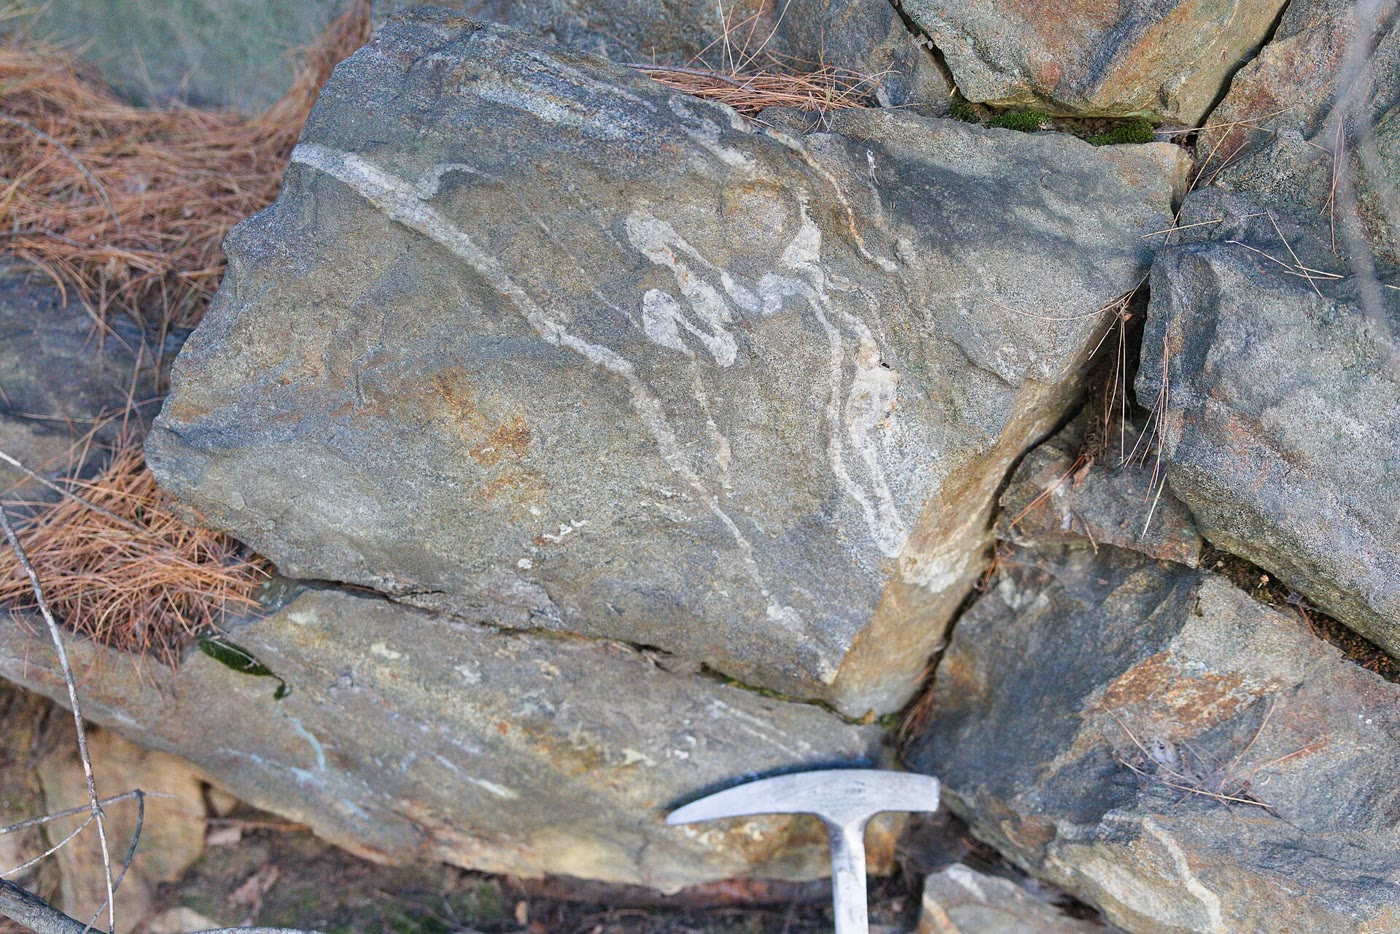
\includegraphics[width=0.62\linewidth]{images/book4/b2-12-migmatite.jpg}
\par\smallskip{\small ميغماتيت في ناشوا، نيوهامبشير: عروق ليوكوسوم فاتحة، مطويّة
مع النيس الرمادي الذي يحويها. ومطرقة الجيولوجي تعطي المقياس. الصورة: \mbox{\textdir TLT Kevin M. Gill, CC BY 4.0}.}
\end{omfigure}

\section{من الميغماتيت إلى البلوتون}\label{sec:b2:crustal-melting:segregation}

على مقياس الحبيبة، تقع أول صهارة على امتداد حدود الحبيبات وفي جيوب صغيرة،
موازية للتورّق في الغالب. وعلى صغرها، تغيّر الصخر: ففي تجارب على
غرانيت منصهر جزئيًا، تنخفض متانة الركام انخفاضًا حادًّا بين خط الصلابة
ونسبة صهارة قدرها \num{0.07}، إذ تتّصل حدود الحبيبات الحاملة للصهارة، ثم تنخفض
من جديد، بنحو أربع رتب مقدار لكن انطلاقًا من قيمة منخفضة أصلًا، حين ينهار الهيكل
البلّوري عند نسب صهارة أعلى. فالقشرة المنصهرة جزئيًا ضعيفة إذن،
ويتجمّع التشوّه فيها ما إن يبدأ الانصهار. والتشوّه بدوره يدفع
\omterm{def:b2:magma-emplacement:magma}{الصهارة}: فتُصرَّف من الأرضية على امتداد حدود حبيبات متّصلة إلى ليوكوسومات موازية
للتورّق، ثم خارج الطبقة المنصهرة عبر ليوكوسومات تقطعها،
وتلتقي هذه في قواطع \cref{ch:b2:magma-emplacement}. ويلخّص الشكل أدناه
المسار من المصدر إلى \omterm{def:b2:magma-emplacement:bodies}{البلوتون}.
% ledger: sawyer01:segregation, rh05:connectivity

\begin{omfigure}
\centering
\begin{tikzpicture}[x=1cm, y=1cm]
\fill[gray!20] (0,0) rectangle (11,1.6);
\fill[gray!8] (0,1.6) rectangle (11,5.2);
\node[font=\scriptsize, anchor=west] at (0.1,0.25) {\foreignlanguage{arabic}{قشرة سفلى ميغماتيتية (المصدر)}};
\foreach \x in {0.6,1.6,2.6,3.6,4.6,5.6,6.6,7.6,8.6,9.6} {
  \draw[white, line width=2.2pt] (\x,0.65) .. controls (\x+0.3,0.75) and (\x+0.5,0.6) .. (\x+0.8,0.7);
  \draw[white, line width=2.2pt] (\x+0.2,1.2) .. controls (\x+0.45,1.3) and (\x+0.6,1.15) .. (\x+0.85,1.25);
}
\foreach \x in {2.8, 5.2, 7.9} {
  \draw[red!70!black, line width=1.4pt] (\x,1.3) .. controls (\x+0.1,2.2) and (\x-0.1,2.9) .. (5.5,3.65);
}
\fill[pink!60, draw=red!70!black, thick] (4.0,3.7) .. controls (4.3,4.6) and (6.7,4.6) .. (7.0,3.7)
  .. controls (6.3,3.4) and (4.7,3.4) .. (4.0,3.7);
\node[font=\scriptsize] at (5.5,4.05) {بلوتون};
\node[font=\scriptsize, anchor=west] at (8.3,2.5) {قواطع};
\draw[->, thick] (8.25,2.5) -- (7.95,2.3);
\node[font=\scriptsize, anchor=west] at (0.1,4.85) {القشرة العليا};
\draw[thick] (0,5.2) -- (11,5.2);
\node[font=\scriptsize, anchor=south east] at (10.9,5.2) {السطح};
\node[font=\scriptsize, align=left, anchor=west] at (9.0,1.05) {الليوكوسومات};
\end{tikzpicture}
\par\smallskip{\small من \omterm{def:b2:crustal-melting:migmatite}{الميغماتيت} إلى \omterm{def:b2:magma-emplacement:bodies}{البلوتون}، تخطيطيًا ودون مقياس رسم: الليوكوسومات
(بالأبيض) في المصدر المنصهر جزئيًا تلتقي في قواطع (بالأحمر) تغذّي بلوتونًا أعلى في
القشرة.}
\end{omfigure}

كم تبقى القشرة منصهرة؟ في الهيمالايا، بدأ \omterm{def:b2:crustal-melting:anatexis}{الأناتكسيس} الواسع الانتشار نحو
30 مليون سنة بعد تصادم الهند مع آسيا، ويعطي زركون الصخور الأناتكسية ومونازيتها
أعمارًا من نحو 25 إلى 15 مليون سنة مضت؛ وقد تغطّي عيّنة واحدة
معظم هذا المدى. فلم يكن انصهار القشرة الهيمالايية حدثًا بل حالة
دامت نحو عشرة ملايين سنة.
% ledger: weinberg16:himalaya

\section{أنماط الغرانيت}\label{sec:b2:crustal-melting:types}

يتذكّر الغرانيت مصدره في كيميائه، وقبل كل شيء في مقدار الألومنيوم الذي
يحويه مقارنةً بما تستطيع فلسباراته أن تأخذه.

\begin{definition}[مؤشر التشبّع بالألومنيوم]\label{def:b2:crustal-melting:asi}
\emph{مؤشر التشبّع بالألومنيوم}\index{مؤشر التشبّع بالألومنيوم} لصخر هو
النسبة المولية
\[\mathrm{A/CNK} = \frac{n(\ce{Al2O3})}{n(\ce{CaO}) + n(\ce{Na2O}) + n(\ce{K2O})},\]
ورفيقه $\mathrm{A/NK} = n(\ce{Al2O3})/[n(\ce{Na2O}) + n(\ce{K2O})]$. ويكون الصخر
\emph{فوق ألوميني}\index{فوق ألوميني} إذا كان $\mathrm{A/CNK} > 1$،
و\emph{ميتاألوميني}\index{ميتاألوميني} إذا كان $\mathrm{A/CNK} < 1 < \mathrm{A/NK}$،
و\emph{فوق قلوي}\index{فوق قلوي} إذا كان $\mathrm{A/NK} < 1$.
\end{definition}
% ledger: moyen17:aluminosity, frost01:asi

\begin{proposition}[ما يقيسه المؤشر]\label{prop:b2:crustal-melting:feldspar}
الصخر الذي يوجد كل كالسيومه وصوديومه وبوتاسيومه في الفلسبارات، ويوجد
كل ألومنيومه في الفلسبارات، يكون له $\mathrm{A/CNK} = 1$. ومن ثَمّ فللصخر \omterm{def:b2:crustal-melting:asi}{فوق الألوميني} ألومنيوم
فائض بعد فلسباراته، محمول في معادن ألومينية (المسكوفيت، والغارنت، والكورديريت،
وسيليكات الألومنيوم)؛ وللصخر \omterm{def:b2:crustal-melting:asi}{الميتاألوميني} كالسيوم فائض، محمول في سيليكات الكالسيوم
(الهورنبلند، والكلينوبيروكسين، والتيتانيت)؛ وللصخر \omterm{def:b2:crustal-melting:asi}{فوق القلوي} صوديوم وبوتاسيوم
فائضان، محمولان في معادن ليس فيها ما يكفي من الألومنيوم للفلسبار (البيروكسين الصودي
والأمفيبول الصودي).
\end{proposition}

\begin{proof}
في صيغة الأكاسيد، الفلسبار البوتاسي هو \ce{K2O.Al2O3.6SiO2}، والألبيت \ce{Na2O.Al2O3.6SiO2}
والأنورثيت \ce{CaO.Al2O3.2SiO2}: ففي كل صيغة \ce{Al2O3} واحد بالضبط مقابل
\ce{K2O} أو \ce{Na2O} أو \ce{CaO} واحد. فأيّ خليط من الثلاثة يكون إذن $n(\ce{Al2O3}) =
n(\ce{CaO}) + n(\ce{Na2O}) + n(\ce{K2O})$، أي $\mathrm{A/CNK} = 1$. وإذا كان
$\mathrm{A/CNK} > 1$، فالألومنيوم يتجاوز ما تستطيع القلويات والكالسيوم ربطه في
فلسبار، ولا بدّ أن يستقرّ الفائض في معادن أخرى. وإذا كان $\mathrm{A/CNK} < 1$ لكن
$\mathrm{A/NK} > 1$، فهناك ما يكفي من الألومنيوم لكل الصوديوم والبوتاسيوم في
فلسبار لكن ليس لكل الكالسيوم، الذي يذهب إلى معادن تحتاج إلى ألومنيوم أقل
لكل كالسيوم مما يحتاج إليه الأنورثيت. وإذا كان $\mathrm{A/NK} < 1$، فحتى القلويات لا يمكن أن تكون كلها في
فلسبار.
\end{proof}

وجد موايان ومعاونوه أن الألومينية هي أنفع مؤشر للتمييز بين غرانيتات
ذات مصادر مختلفة؛ ويستعمل فروست ومعاونوه المؤشر نفسه، مع تصحيح صغير
للفوسفور، محورًا من المحاور الثلاثة لتصنيفهم للصخور
الغرانيتية.
% ledger: moyen17:aluminosity, frost01:asi

\begin{omfigure}
\centering
\begin{tikzpicture}
\begin{axis}[omrecord, width=0.72\linewidth, height=7cm,
  xmin=0.4, xmax=1.5, ymin=0.4, ymax=3.5, xlabel={النسبة المولية \babelsublr{A/CNK}}, ylabel={النسبة المولية \babelsublr{A/NK}},
  tick label style={font=\scriptsize}, label style={font=\small}]
\addplot[fill=gray!15, draw=none] coordinates {(0.4,0.4) (1.5,1.5) (1.5,0.4) (0.4,0.4)};
\addplot[thick, black!70] coordinates {(1,0.4) (1,3.5)};
\addplot[thick, black!70] coordinates {(0.4,1) (1.5,1)};
\node[font=\scriptsize, anchor=north east] at (axis cs:1.48,3.45) {فوق ألوميني};
\node[font=\scriptsize, anchor=west] at (axis cs:0.62,2.6) {ميتاألوميني};
\node[font=\scriptsize, anchor=south west] at (axis cs:0.42,0.45) {فوق قلوي};
\addplot[only marks, mark=*, mark size=2pt, blue!70!black, nodes near coords,
  point meta=explicit symbolic, every node near coord/.style={font=\scriptsize, anchor=west}]
  coordinates {(0.539,3.196)[BHVO-2] (0.877,1.694)[AGV-2] (0.993,1.135)[SRM 278]};
\addplot[only marks, mark=square*, mark size=2pt, red!70!black]
  coordinates {(1.261,1.377) (0.809,0.844)};
\node[font=\scriptsize, red!70!black, anchor=south] at (axis cs:1.261,1.45) {\foreignlanguage{arabic}{صهارة من النمط S}};
\node[font=\scriptsize, red!70!black, anchor=north] at (axis cs:0.809,0.79) {غرانيت فوق قلوي};
\end{axis}
\end{tikzpicture}
\par\smallskip{\small مخطّط شاند. الدوائر الزرقاء: ثلاث مواد مرجعية، بازلت من
هاواي \babelsublr{(BHVO-2)}، وأنديزيت \babelsublr{(AGV-2)}، وأوبسيديان ذو تركيب غرانيتي \babelsublr{(SRM 278)}،
محسوبة من محتوياتها المنشورة من الأكاسيد. والمربعات الحمراء: غرانيتان مخترعان مستعملان في
هذا الفصل. والمثلث الرمادي لا يمكن بلوغه، لأن \babelsublr{A/CNK} لا تتجاوز أبدًا \babelsublr{A/NK}.}
\end{omfigure}
% ledger: usgs:bhvo2-major, usgs:agv2-major, nist278:majors

الكيمياء تتبع المصدر. ففي عام 1974، لاحظ تشابل ووايت أن غرانيتات حزام لاكلان
الطيّ، باستثناء أشدّ الصخور فلسيةً، تنقسم إلى مجموعتين متميّزتين،
وفسّراهما على أنهما صهارتان لنوعين من الصخور المصدر: صخور نارية أقدم وصخور رسوبية. وحلمأة الفلسبارات، التي عرضها مجلد السنة
الأولى، تحمل الصوديوم والكالسيوم بعيدًا في المحلول وتُبقي الألومنيوم في الطين: فالأطيان المكوّنة
من هذا الطين غنية بالألومنيوم، وكذلك صهاراتها.
% ledger: cw01:is-types

\begin{definition}[تصنيف أنماط الغرانيت]\label{def:b2:crustal-melting:types}
\emph{غرانيت النمط I}\index{غرانيت النمط I} غرانيت كان مصدره في الغالب
صخرًا ناريًا أقدم، و\emph{غرانيت النمط S}\index{غرانيت النمط S} غرانيت كان مصدره
في الغالب صخرًا رسوبيًا (رسوبيًا متحوّلًا)، وغرانيت النمط M غرانيت مشتقّ من
الوشاح. أمّا \emph{غرانيت النمط A}\index{غرانيت النمط A} فيُعرَّف بكيميائه
وإطاره لا بمصدره: حديدي وبوتاسي، شديد الإغناء بالعناصر غير المتوافقة،
ومتموضع في أطر مستقرة داخل الصفائح، أو خلف الأقواس، أو بعد التصادم.
\end{definition}
% ledger: johansson23:a-type, cw01:is-types

\omterm{def:b2:crustal-melting:types}{غرانيتات النمط S} فوق ألومينية، بنوعين من الميكا أو بالكورديريت؛ وغرانيتويدات النمط A
ميتاألومينية في الغالب، وبعضها \omterm{def:b2:crustal-melting:asi}{فوق ألوميني}. لكن تحليلًا واحدًا قد يضلّل: فكل
متتالية غرانيتويدية تنتهي قرب تركيب الحدّ الأدنى الغرانيتي، الفاتح اللون \omterm{def:b2:crustal-melting:asi}{وفوق الألوميني}
باعتدال، فلا تكون العيّنة فوق الألومينية دليلًا على أن القشرة انصهرت. وما يميّز
المتتاليات هو شكل اتجاهها في مخطّط شاند: فمتتالية القوس تبلغ
الحدّ الأدنى على امتداد مصفوفة شديدة الانحدار من \babelsublr{A/NK} مرتفعة و\babelsublr{A/CNK} منخفضة، ومتتالية النمط S الفقيرة بالكالسيوم
على امتداد مصفوفة تكون فيها \babelsublr{A/NK} قريبة من \babelsublr{A/CNK}. ولم يُتوصّل إلى إجماع على مصدر
صهارات النمط A: فأحد النماذج يصنعها من بازلت مبطَّن، متطوّر بالتبلور،
\omterm{def:b2:mantle-melting:melting}{والانصهار الجزئي} واستيعاب القشرة.
% ledger: moyen17:trends, frost01:asi, johansson23:a-type

\begin{definition}[الليوكوغرانيت]\label{def:b2:crustal-melting:leucogranite}
\emph{الليوكوغرانيت}\index{الليوكوغرانيت} غرانيت فاتح اللون، يكاد يخلو من
المعادن الداكنة؛ وتحمل الليوكوغرانيتات فوق الألومينية في أحزمة التصادم المسكوفيت، وحده أو
مع البيوتيت.
\end{definition}
% ledger: moyen17:aluminosity, pdh98:himalaya

الليوكوغرانيتات فوق الألومينية الحاملة للمسكوفيت في أحزمة التصادم لها تراكيب قريبة
من سوائل الانصهار بحضور الماء أو \omterm{def:b2:crustal-melting:reactions}{انصهار نزع الماء} من المسكوفيت، عند درجات حرارة قرب
\qty{700}{\celsius} حيث يستطيع زركون المصدر ومونازيته البقاء والانتقال
إلى \omterm{def:b2:magma-emplacement:magma}{الصهارة} بلّورات غريبة؛ أمّا الغرانيتات فوق الألومينية الحاملة للكورديريت فتأتي من
تفكّك البيوتيت الأسخن، عند 800 إلى \qty{850}{\celsius}. والليوكوغرانيتات الهيمالايية،
ببصمتها النظيرية القشرية القوية، تنتمي إلى هذه العائلة
(\cref{ch:b2:himalaya-andes}).
% ledger: moyen17:aluminosity, weinberg16:himalaya

\begin{omfigure}
\centering
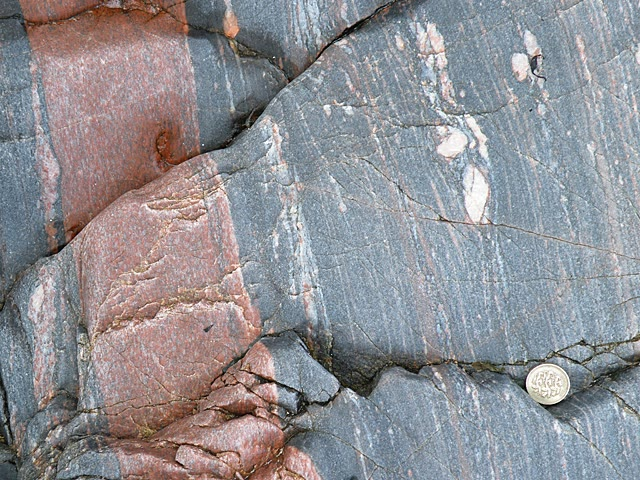
\includegraphics[width=0.5\linewidth]{images/book4/b2-12-leucogranite-vein.jpg}
\par\smallskip{\small عرق ليوكوغرانيتي وردي يقطع نيسًا رماديًا شريطيًا؛ والقطعة النقدية تعطي
المقياس. الصورة: \mbox{\textdir TLT Anne Burgess (Geograph), CC BY-SA 2.0}.}
\end{omfigure}

\section{الغرانيتات ونموّ القارات}\label{sec:b2:crustal-melting:time}

نوعان من الأماكن يصنعان معظم الغرانيت. فوق نطاقات الاندساس، تتكوّن قشرة القوس
بتمايز صهارات مافية آتية من الوشاح، والحرارة المتاحة ليست إلا ما تجلبه هذه
الصهارات. وبعد التصادم، تكون القشرة المثخنة نظامًا شديد السخونة: فهي تنصهر على
نطاق واسع، عند درجة حرارة منخفضة حيث يسمح الماء أو المسكوفيت بذلك وعند درجة حرارة أعلى
بتفكّك البيوتيت، وهذه الغرانيتات المشتقّة من القشرة تعيد تدوير قشرة
كانت موجودة. وتبلغ صهارات الوشاح القشرة هناك أيضًا، بكميات كبيرة بما يكفي، كما يرى موايان
ومعاونوه، لتجعل أحزمة أواخر التكوّن الجبلي مساهمًا مهمًّا في نموّ
القشرة. فكون الغرانيت يضيف إلى القارات أو يعيد تشكيلها فقط هو إذن مسألة
مصدره، الذي تجيب عنه نظائره (\cref{ch:b2:isotope-geochemistry})؛ أمّا غرانيتات
الأرض المبكرة، المختلفة جدًّا عن هذه، فهي موضوع
\cref{ch:b2:precambrian-earth}.
% ledger: moyen17:settings

\section{التمارين}\label{sec:b2:crustal-melting:exercises}

الكتل المولية (\unit{\gram\per\mole}): \ce{Al2O3} 101.96، \ce{CaO} 56.08، \ce{Na2O} 61.98،
\ce{K2O} 94.20، \ce{H2O} 18.02؛ والكتل الذرية: الهيدروجين 1.008، والأكسجين 16.00، والصوديوم 22.99، والمغنيسيوم 24.31،
والألومنيوم 26.98، والسيليكون 28.09، والبوتاسيوم 39.10، والكالسيوم 40.08. وخذ $g = \qty{9.81}{\metre\per\second\squared}$.

\begin{exercise}[$\star$]\label{exo:b2:crustal-melting:1}
تحوي المادة المرجعية الأنديزيتية \babelsublr{AGV-2}، بالغرام لكل \qty{100}{\gram}،
\ce{Al2O3} 17.03، و\ce{CaO} 5.15، و\ce{Na2O} 4.204، و\ce{K2O} 2.898.
(أ) احسب نسبتيها \babelsublr{A/CNK} و\babelsublr{A/NK}. (ب) صنّفها، وسمِّ معدنًا ينبغي أن يحمل
كالسيومها الفائض.
\end{exercise}
% ledger: usgs:agv2-major

\begin{exercise}[$\star$]\label{exo:b2:crustal-melting:2}
تحوي ثلاثة غرانيتات، إلى جانب الكوارتز والفلسبارات: (أ) المسكوفيت والبيوتيت والغارنت؛
(ب) الهورنبلند والبيوتيت والتيتانيت؛ (ج) الإيجيرين، وهو بيروكسين صوديوم--حديد
\ce{NaFeSi2O6}، وأمفيبولًا صوديًا. صنّف كلًّا منها بتشبّعه بالألومنيوم، وقل
أيّها يمكن أن يكون \omterm{def:b2:crustal-melting:types}{غرانيتًا من النمط S}.
\end{exercise}

\begin{exercise}[$\star$]\label{exo:b2:crustal-melting:3}
لقشرة كثافتها \qty{2800}{\kilogram\per\cubic\metre} تدرّج حراري أرضي خطّي
$T = \qty{10}{\celsius} + (\qty{20}{\celsius\per\kilo\metre})\,z$. بين 2
و\qty{10}{kbar}، قرّب خط صلابة الغرانيت الرطب بالخط المستقيم المارّ بالنقطتين
\babelsublr{(\qty{680}{\celsius}, \qty{2}{kbar})} و\babelsublr{(\qty{620}{\celsius}, \qty{10}{kbar})}. عند أيّ
عمق ودرجة حرارة وضغط يلتقيه التدرّج الحراري الأرضي؟
\end{exercise}
% ledger: sw81:wet-solidus

\begin{exercise}[$\star$]\label{exo:b2:crustal-melting:4}
يحمل نيس بيوتيتي رمادي طبقات بيضاء سمكها سنتيمتر من الكوارتز والفلسبار، موازية
لتورّقه، يحدّ كلًّا منها شريط أسود رقيق من البيوتيت؛ وبين الطبقات يبدو
النيس عاديًا. (أ) سمِّ الطبقات البيضاء والأشرطة السوداء والنيس العادي.
(ب) هل الصخر ميتاتكسيت أم دياتكسيت، وما بنيته؟ (ج) على بُعد بضع مئات
من الأمتار، اختفى التطبّق: صخر مخطّط شبيه بالغرانيت يحوي أشباحًا باهتة من
النيس. ما الذي تغيّر؟
\end{exercise}
% ledger: scmr:migmatite, bgs99:migmatite

\begin{exercise}[$\star\star$]\label{exo:b2:crustal-melting:5}
خذ البيوتيت فلوغوبيتًا، \ce{KMg3AlSi3O10(OH)2}. (أ) احسب كتلته المولية
والنسبة الكتلية للماء الذي يحرّره (مجموعتا الهيدروكسيل فيه تعطيان \ce{H2O} واحدًا).
(ب) نيس فيه \qty{25}{\percent} بيوتيت كتليًا ينصهر \omterm{def:b2:crustal-melting:reactions}{بانصهار نزع الماء} من البيوتيت
إلى صهارة تحوي \qty{4.0}{\percent} ماء. باستعمال
\cref{prop:b2:crustal-melting:water}، جد نسبة \omterm{def:b2:magma-emplacement:magma}{الصهارة}، وقارنها
بالنسب الموجودة في تجارب \omterm{def:b2:crustal-melting:reactions}{انصهار نزع الماء} من البيوتيت.
\end{exercise}
% ledger: bk99:migmatites

\begin{exercise}[$\star\star$]\label{exo:b2:crustal-melting:6}
تحوي مئة غرام من الغرانيت \qty{30}{\gram} من الفلسبار البوتاسي \ce{KAlSi3O8}،
و\qty{35}{\gram} من الألبيت \ce{NaAlSi3O8}، و\qty{5}{\gram} من الأنورثيت \ce{CaAl2Si2O8}،
و\qty{25}{\gram} من الكوارتز و\qty{5}{\gram} من المسكوفيت \ce{KAl3Si3O10(OH)2}.
(أ) احسب الكتل المولية للمعادن الألومينية الأربعة. (ب) احسب كميات
\ce{Al2O3} و\ce{CaO} و\ce{Na2O} و\ce{K2O} في الصخر، ونسبته \babelsublr{A/CNK}. (ج) أيّ
معدن يجعل الصخر \omterm{def:b2:crustal-melting:asi}{فوق ألوميني}؟
\end{exercise}

\begin{exercise}[$\star\star$]\label{exo:b2:crustal-melting:7}
عتبة بازلتية متداخلة عند \qty{1200}{\celsius} تتبلور كليًا وتبرد إلى
\qty{850}{\celsius}، فتحرّر حرارة كامنة قدرها \qty{900}{\mega\joule\per\cubic\metre}.
والقشرة المحيطة بها، عند \qty{650}{\celsius}، تُسخَّن إلى \qty{850}{\celsius}
وينصهر \qty{20}{\percent} منها، بالحرارة الكامنة نفسها لكل وحدة حجم من \omterm{def:b2:magma-emplacement:magma}{الصهارة}. ولكلا
الصخرين سعة حرارية قدرها \qty{2.5}{\mega\joule\per\cubic\metre\per\kelvin}. باستعمال
\cref{prop:b2:crustal-melting:heat}، كم مترًا مكعبًا من القشرة يستطيع متر مكعب واحد
من البازلت أن يعالج على هذا النحو؟ وما الذي تتجاهله النتيجة؟
\end{exercise}
% ledger: delaney86b4:properties

\begin{exercise}[$\star\star$]\label{exo:b2:crustal-melting:8}
المادة المرجعية الأوبسيديانية \babelsublr{SRM 278} مصدَّقة بالقيم: \ce{Al2O3}
$14.15 \pm 0.15$، و\ce{CaO} 0.983، و\ce{Na2O} 4.84، و\ce{K2O} 4.16 (\unit{\percent}
كتليًا). (أ) احسب نسبتيها \babelsublr{A/CNK} و\babelsublr{A/NK} وصنّفها. (ب) أعد حساب \babelsublr{A/CNK} بطرفي
عدم اليقين في \ce{Al2O3}. هل التصنيف متين؟
\end{exercise}
% ledger: nist278:majors

\begin{exercise}[$\star\star$]\label{exo:b2:crustal-melting:9}
عند \qty{800}{\celsius}، تحوي صهارة هابلوغرانيتية مشبعة بالماء \qty{7.45}{\percent}
ماءً تحت \qty{3}{kbar}، و8.94 تحت \qty{4}{kbar}، و9.97 تحت \qty{5}{kbar}، و13.82 تحت
\qty{8}{kbar}. (أ) لائم خطًا مستقيمًا مع هذه النقاط الأربع بالمربعات الصغرى وقارن
ميله بالقيمة \qty{1.27}{\percent} لكل كيلوبار التي ذكرها المجرّبون.
(ب) تنبّأ بمحتوى التشبّع تحت \qty{6}{kbar}. (ج) ما أقل كتلة من \omterm{def:b2:magma-emplacement:magma}{الصهارة}
تستطيع حمل \qty{10}{\gram} من الماء تحت \qty{6}{kbar}؟ (د) لماذا لا ينبغي استعمال الخط
تحت \qty{15}{kbar}؟
\end{exercise}
% ledger: holtz95:solubility

\begin{exercise}[$\star\star\star$]\label{exo:b2:crustal-melting:10}
قرّب خط صلابة \omterm{def:b2:crustal-melting:reactions}{انصهار نزع الماء} لشيست مسكوفيتي بالخط المستقيم
المارّ بالنقطتين \babelsublr{(\qty{750}{\celsius}, \qty{6}{kbar})} و\babelsublr{(\qty{800}{\celsius}, \qty{10}{kbar})}،
وهما طرفا الحصرين التجريبيين. يصعد شيست عند \qty{770}{\celsius} من
\qty{10}{kbar} دون أن يكسب حرارة أو يفقدها. (أ) عند أيّ ضغط يبلغ
خط الصلابة؟ (ب) بعد ذلك، تتبع درجة حرارته خط الصلابة نزولًا، والحرارة اللازمة للانصهار آتية
من تبريده هو. مع سعة حرارية قدرها \qty{2.5}{\mega\joule\per\cubic\metre\per\kelvin}
وحرارة كامنة قدرها \qty{900}{\mega\joule\per\cubic\metre}، ما النسبة الحجمية للصهارة التي
تكوّنت حين يبلغ \qty{6}{kbar}؟ (ج) قارن بالظروف المقترحة
لليوكوغرانيت الهيمالايي.
\end{exercise}
% ledger: pdh98:himalaya, delaney86b4:properties

\begin{exercise}[$\star\star\star$]\label{exo:b2:crustal-melting:11}
تنتشر الحرارة على مسافة $\ell$ في زمن من رتبة $\ell^2/\kappa$. مع
$\kappa = \qty{1e-6}{\square\metre\per\second}$، قدّر الزمن اللازم لحرارة
عتبة سمكها \qty{2}{km}، ولحرارة طبقة مبطَّنة سمكها \qty{10}{km}، كي تنتشر على
سمكها هي. قارن بالملايين العشرة من السنين للأناتكسيس الهيمالايي: هل يستطيع
حدث تبطين واحد أن يفسّره؟
\end{exercise}
% ledger: delaney86b4:properties, weinberg16:himalaya

\begin{exercise}[$\star\star\star$]\label{exo:b2:crustal-melting:12}
يُحلَّل ميغماتيت ستروماتي: \omterm{def:b2:crustal-melting:migmatite}{الليوكوسوم} \ce{K2O} \qty{5.0}{\percent}، و\ce{MgO}
\qty{0.20}{\percent}؛ \omterm{def:b2:crustal-melting:migmatite}{والميلانوسوم} \ce{K2O} \qty{2.0}{\percent}، و\ce{MgO}
\qty{4.0}{\percent}؛ والميزوسوم، المأخوذ على أنه الصخر الأم غير المنصهر، \ce{K2O}
\qty{2.75}{\percent}، و\ce{MgO} \qty{3.05}{\percent} (كلها كتليًا). (أ) إذا كان
النيوسوم قد تكوّن من الصخر الأم دون كسب ولا فقد، فما النسبة الكتلية منه التي هي
ليوكوسوم؟ (ب) تحقّق من الجواب بواسطة \ce{MgO}. (ج) على المكشف لا يشكّل \omterm{def:b2:crustal-melting:migmatite}{الليوكوسوم} إلا
\qty{10}{\percent} من النيوسوم كتليًا. كم غرامًا من \omterm{def:b2:magma-emplacement:magma}{الصهارة} غادر لكل
\qty{100}{\gram} من الصخر الأم؟
\end{exercise}

\begin{problem}[{مسألة نهاية الأسبوع --- بلوتون من ميكا منصهرة}]\label{pb:b2:crustal-melting:1}
شيست مكوّن من \qty{20}{\percent} مسكوفيت، و\qty{15}{\percent} بيوتيت،
و\qty{30}{\percent} كوارتز، و\qty{30}{\percent} بلاجيوكليز، و\qty{5}{\percent} معادن
أخرى (كتليًا؛ صخر مخترع) يقع عند قاعدة قشرة مضاعفة بالتكديس، وهي
الحالة المنمذجة في \cref{ch:b2:pt-paths}. قد ينصهر ويغذّي بلوتونًا غرانيتيًا. المعطيات:
الكتل الذرية والمولية في رأس التمارين؛ ويمرّ خط صلابة الغرانيت الرطب
بالنقاط \babelsublr{(\qty{680}{\celsius}, \qty{2}{kbar})} و\babelsublr{(\qty{620}{\celsius}, \qty{10}{kbar})}
و\babelsublr{(\qty{605}{\celsius}, \qty{15.3}{kbar})} و\babelsublr{(\qty{670}{\celsius}, \qty{27}{kbar})}؛
ومحتوى التشبّع بالماء لصهارة غرانيتية عند \qty{800}{\celsius} هو \qty{9.97}{\percent} تحت
\qty{5}{kbar} و\qty{13.82}{\percent} تحت \qty{8}{kbar}. وتتبع قاعدة القشرة المثخنة في النموذج ما يلي:

\smallskip
\begin{center}\small
\begin{tabular}{l|ccccccccccc}
\mbox{\textdir TLT $t$ (\unit{Myr})} & 0 & 10 & 20 & 30 & 40 & 50 & 60 & 70 & 80 & 90 & 100\\ \hline
\mbox{\textdir TLT $T$ (\unit{\celsius})} & 595 & 656 & 734 & 795 & 845 & 885 & 909 & 914 & 900 & 867 & 814\\
\mbox{\textdir TLT $P$ (\unit{kbar})} & 19.2 & 19.2 & 19.2 & 19.2 & 17.9 & 16.5 & 15.1 & 13.7 & 12.4 & 11.0 & 9.6
\end{tabular}
\end{center}
\smallskip

\noindent\textbf{الجزء الأول --- الماء من الميكا.}
\begin{enumerate}
\item احسب الكتلة المولية للمسكوفيت \ce{KAl3Si3O10(OH)2}.
\item مجموعتا الهيدروكسيل فيه تعطيان \ce{H2O} واحدًا. ما النسبة الكتلية من المعدن التي
تتحرّر ماءً؟
\item كم من الماء يحرّر مسكوفيت كيلوغرام واحد من الشيست؟
\item بالاستيفاء الخطّي، ما محتوى \omterm{def:b2:magma-emplacement:magma}{الصهارة} من الماء عند التشبّع تحت
\qty{7}{kbar}؟ وما أقل نسبة صهارة يستطيع ماء المسكوفيت عندئذ أن يصنعها؟
\item صهارة \omterm{def:b2:crustal-melting:reactions}{انصهار نزع الماء} بعيدة عن التشبّع؛ خذ محتواها من الماء
\qty{6.0}{\percent}. ما نسبة \omterm{def:b2:magma-emplacement:magma}{الصهارة} التي يصنعها المسكوفيت؟
\item في تجارب على ميتابيليت ثنائي الميكا تحت \qty{10}{kbar}، لم يعطِ تفاعل المسكوفيت
إلا 1 إلى \qty{2}{\percent} من \omterm{def:b2:magma-emplacement:magma}{الصهارة}. اذكر سببين قد يجعلان صخرًا حقيقيًا يصنع صهارة
أقل من جوابك عن السؤال~5.
\end{enumerate}

\noindent\textbf{الجزء الثاني --- تسخين المصدر.}
\begin{enumerate}[resume]
\item في \cref{ch:b2:pt-paths}، يبلغ الصخر المتروك في منتصف القشرة ذروته عند \qty{593}{\celsius}
و\qty{7.8}{kbar}. ما خط الصلابة الرطب تحت \qty{7.8}{kbar}؟ وهل يستطيع ذلك الصخر أن ينصهر، حتى
مع ماء حرّ؟
\item بالاستيفاء بين 15.3 و\qty{27}{kbar}، جد خط الصلابة الرطب عند ضغط
القاعدة بعد التكديس مباشرة. هل القاعدة فوقه عند $t = 0$؟ وعند $t = \qty{10}{Myr}$؟
\item ما الذي يحدّ انصهار القاعدة عند $t = \qty{10}{Myr}$، ولماذا يتوقّف
سريعًا؟
\item متى تتجاوز القاعدة \qty{800}{\celsius}، وهي الطرف الأعلى لحصر
المسكوفيت؟
\item يمتدّ حصر الأمفيبول من 875 إلى \qty{925}{\celsius} تحت 10 إلى \qty{12.5}{kbar}.
متى تدخل القاعدة مجال الضغط هذا، وعند أيّ درجة حرارة؟
\item متى تبلغ القاعدة \qty{10}{kbar}، وهو أعلى مجال الضغط في
تجارب المسكوفيت، وكم تكون حرارتها عندئذ؟ وأيّ المعادن المائية في الشيست يمكن أن
يبقى موجودًا؟
\end{enumerate}

\noindent\textbf{الجزء الثالث --- أيّ صهارة؟}
تعطي \omterm{def:b2:magma-emplacement:magma}{الصهارة}، بعد تبلورها، ليوكوغرانيتًا (تحليل مخترع) فيه، بالنسب
\unit{\percent} الكتلية، \ce{Al2O3} 15.0، و\ce{CaO} 0.55، و\ce{Na2O} 3.4، و\ce{K2O} 4.9.
\begin{enumerate}[resume]
\item احسب كميات الأكاسيد الأربعة في \qty{100}{\gram} من الصخر.
\item احسب نسبته \babelsublr{A/CNK}.
\item احسب نسبته \babelsublr{A/NK} وصنّف \omterm{def:b2:crustal-melting:leucogranite}{الليوكوغرانيت}.
\item هل هو غرانيت من النمط I أم من النمط S؟ سمِّ معدنين ينبغي أن يحملا ألومنيومه
الفائض.
\item كم مولًا من \ce{Al2O3} لكل \qty{100}{\gram} يبقى فائضًا بعد
الفلسبارات؟ إذا ذهب كله إلى المسكوفيت، الذي يحوي \ce{Al2O3} واحدًا زائدًا لكل وحدة
صيغة مقارنةً بالفلسبار البوتاسي، فكم غرامًا من المسكوفيت تحوي \qty{100}{\gram} من الغرانيت؟
\item للأوبسيديان \babelsublr{SRM 278} النسبة \mbox{\textdir TLT A/CNK $= 0.993$}. هل يمكن أن يأتي \omterm{def:b2:crustal-melting:leucogranite}{الليوكوغرانيت} والأوبسيديان
من النوع نفسه من المصادر؟
\end{enumerate}

\noindent\textbf{الجزء الرابع --- كم من القشرة؟}
بلوتون مخترع من هذا \omterm{def:b2:crustal-melting:leucogranite}{الليوكوغرانيت} حجمه \qty{1000}{\cubic\kilo\metre}.
خذ \qty{2650}{\kilogram\per\cubic\metre} للغرانيت
و\qty{2800}{\kilogram\per\cubic\metre} للشيست؛ وافترض أن \qty{70}{\percent} من
\omterm{def:b2:magma-emplacement:magma}{الصهارة} تغادر مصدرها وأن كل ماء \omterm{def:b2:magma-emplacement:magma}{الصهارة} يفلت حين تتبلور.
\begin{enumerate}[resume]
\item ما كتلة \omterm{def:b2:magma-emplacement:bodies}{البلوتون}؟
\item ما كتلة \omterm{def:b2:magma-emplacement:magma}{الصهارة} (بمائها البالغ \qty{6.0}{\percent}) التي احتاج إليها؟
\item باستعمال نسبة \omterm{def:b2:magma-emplacement:magma}{الصهارة} في السؤال~5، ما كتلة الشيست التي كان يجب أن تنصهر؟
\item ما حجم ذلك الشيست؟
\item إذا كان المصدر طبقة سمكها \qty{5}{km}، فعلى أيّ مساحة انصهر؟
\item لو استُعملت بدلًا من ذلك أقل نسبة صهارة في السؤال~4، فكم مرة يكبر
المصدر؟ أعطِ حجم قشرة المصدر المنصهرة لصنع \omterm{def:b2:magma-emplacement:bodies}{البلوتون}، بوحدة
\unit{\cubic\kilo\metre}، من السؤال~22.
\end{enumerate}
\end{problem}
